\documentclass[tikz, preview]{standalone}

\usepackage{tikz}
\usepackage[all,2cell]{xy}
\usetikzlibrary{matrix,arrows,shapes,decorations.markings,decorations.pathreplacing}
\definecolor{rewritecolor}{rgb}{0,.9,1}
\tikzset{rewritenode/.style={shape=circle,fill=rewritecolor,scale=0.25,font=\Huge}}
\tikzset{RWopen/.style={shape=circle,draw=black,fill=white,scale=0.5,font=\Huge}}
\tikzset{RWclosed/.style={shape=circle,fill=black,scale=0.5,font=\Huge}}
\tikzset{CDnode/.style={shape=circle,fill=white,scale=.5}}
\tikzset{zxgreen/.style={shape=circle,draw,thick,fill=green}}
\tikzset{zxred/.style={shape=circle,draw,thick,fill=red}}
\tikzset{zxyellow/.style={shape=rectangle,draw,thick,fill=yellow}}
\tikzset{zxdiamond/.style={shape=diamond,fill=black,inner sep=2.75pt}}
\tikzset{->-/.style={decoration={markings,mark=at position .5 with {\arrow{>}}},postaction={decorate}}}

\begin{document}

\[
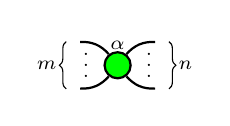
\begin{tikzpicture}
\node [zxgreen,label={[shift={(0,-0.1)}]\scriptsize $\alpha$}] (v1) at (0,0) {};
\node (v2) at (-0.6,0.3) {};
\node (v3) at (-0.6,-0.3) {};
\node (v4) at (0.6,0.3) {};
\node (v5) at (0.6,-0.3) {};
\node at (-0.4,0.1) {\scriptsize $\vdots$};
\node at (0.4,0.1) {\scriptsize $\vdots$};
\draw  (v1) edge [thick,bend right=25] (v2);
\draw  (v1) edge [thick,bend left=25] (v3);
\draw  (v1) edge [thick,bend left=25] (v4);
\draw  (v1) edge [thick,bend right=25] (v5);
\draw[decoration={brace,mirror,raise=5pt},decorate]
	(v2.east) -- node[left=5pt] {\scriptsize $m$} (v3.east); 
\draw[decoration={brace,raise=5pt},decorate]
	(v4.west) -- node[right=5pt] {\scriptsize $n$} (v5.west); 
\end{tikzpicture}
\]



\end{document}
